\section{Introduction to Excel}
%\addcontentsline{toc}{chapter}{Appendix: Introduction to Excel}

%\makelabheader

\bigskip

Microsoft Excel is the spreadsheet program we will use for some of our
data analysis and graphing.  It is a powerful and easy-to-use
application for graphing, fitting, and manipulating data. In this
appendix, I will briefly describe how to use Excel to do some useful
tasks.  

\subsection{Data and formulae}

The figure below shows a sample Excel spreadsheet containing data
from a made-up experiment.  The experimenter was trying to measure
the density of a certain material by taking a set of cubes
made of the material and measuring their masses and the lengths of
the sides of the cubes.  The first two columns contain her measured
results.  \textbf{Note that the top of each column contains both
a description of the quantity contained in that column and its units.}
You should make sure that all of the columns of your data tables do as well.
You should also make sure that the whole spreadsheet has a descriptive
title and your names at the top.

In the third column, the experimenter has figured out the volume
of each of the cubes, by taking the cube of the length of a side.
To avoid repetitious calculations, she had Excel do this automatically.
She entered the formula ``=B3$\wedge$3'' (without the quotes) into cell C3.
Note the equals sign, which indicates to Excel that a formula is coming.
The $\wedge$ sign stands for raising to a power, so this
formula says ``take the value in cell B3 and raise it to the power 3.''
After entering a formula
into a cell, you can grab the square in the lower right corner of the
cell with the mouse and drag it down the column.  This will copy
the cell, making the appropriate changes, into the rest of the column.
For instance, in this case, cell C4 contains the formula ``=B4$\wedge$3,''
and so forth.

Column D was similarly produced with a formula that divides the
mass in column A by the volume in column C.

At the bottom of the spreadsheet we find the mean and standard
deviation of the calculated densities (that is, of the numbers
in cells D3 through D6). For those who don't know, the mean
is just the average, and the 
standard deviation is a measure of how widely scattered the
individual numbers are about the average. The standard deviation
is often used to characterize the margin of error in a measurement.
 The mean and standard deviation were computed
using the formulae ``=average(D3:D6)'' and ``=stdev(D3:D6)''.


{\par\centering \resizebox{5in}{!}{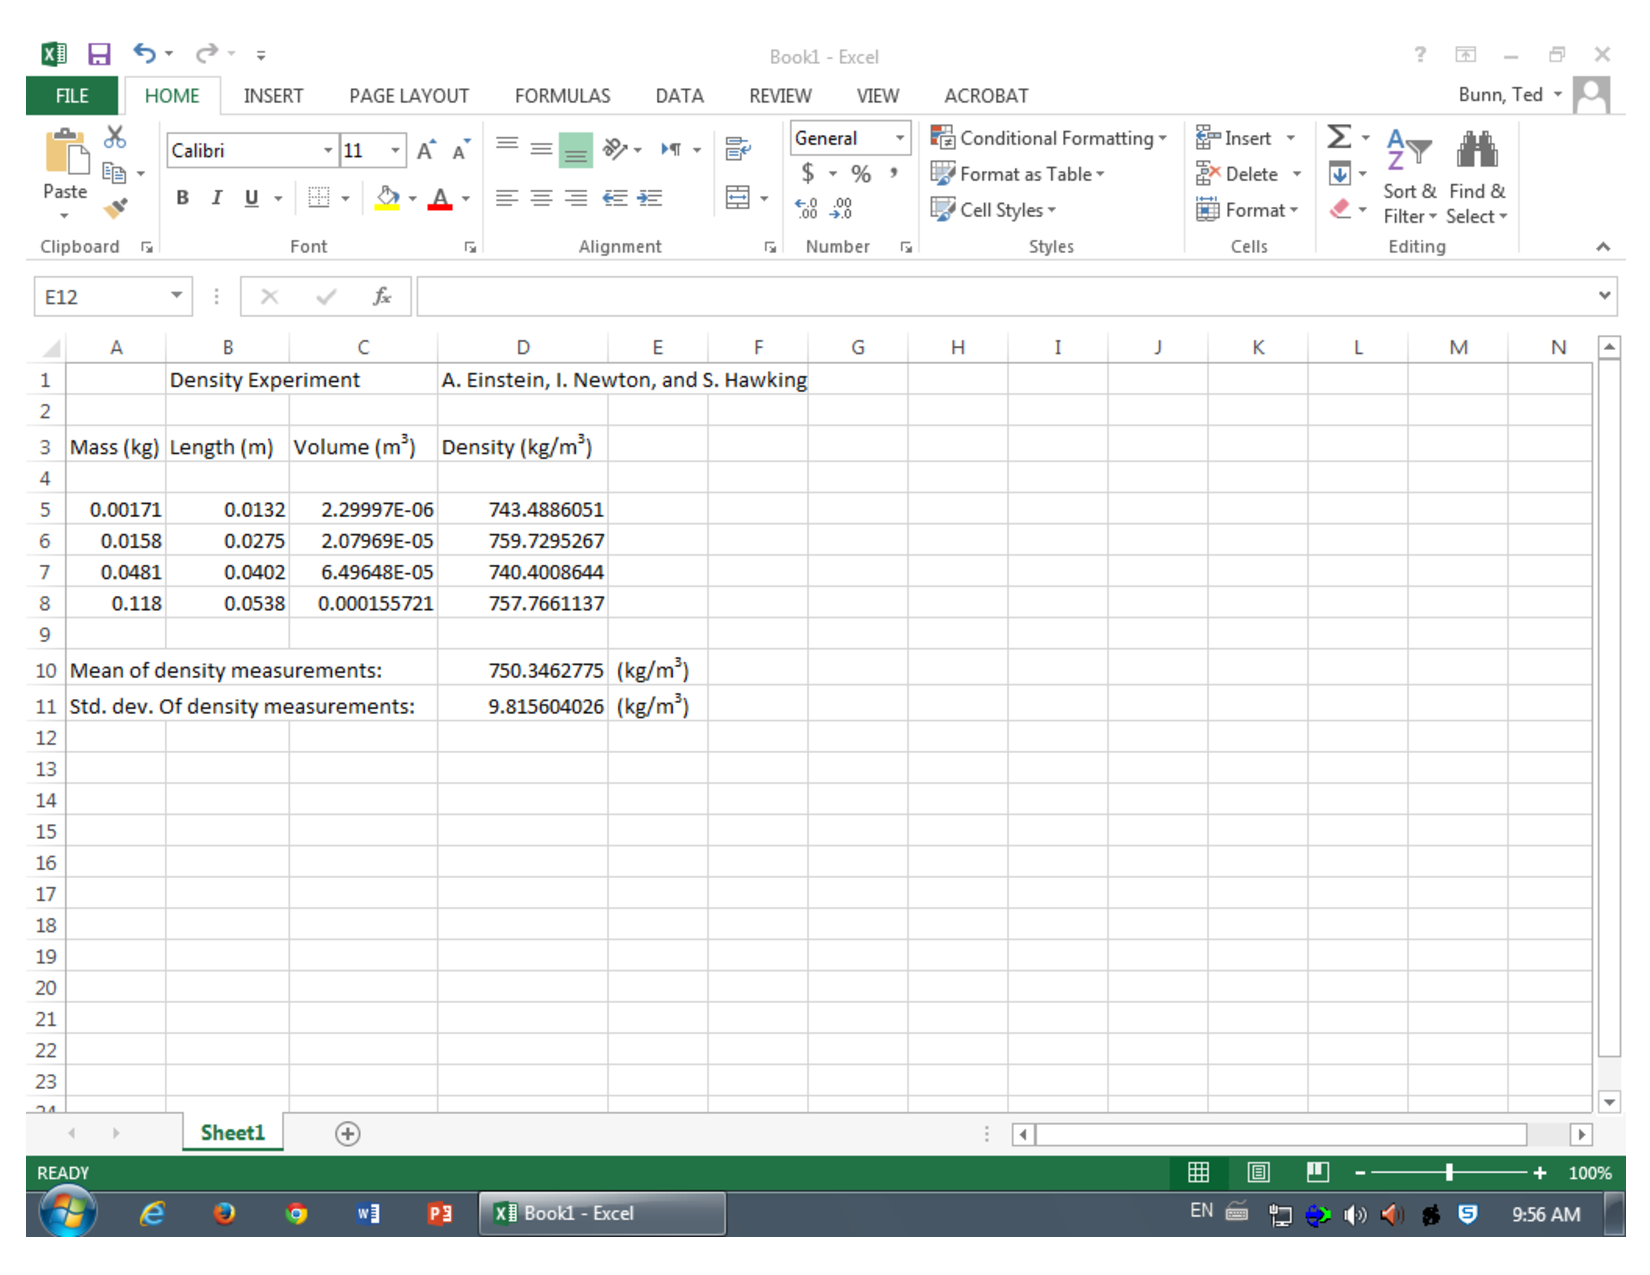
\includegraphics{appendices/excel/densityspreadsheet.pdf}} \par}


\subsection{Graphs}

Here's how to make graphs in Excel.  First, use the mouse
to select the columns of numbers you want to graph.  (If the two
columns aren't next to each other, select the first one, then hold
down the control key while selecting the second one.)
Then click on the ``Insert'' tab at the top of the screen. The
graphs we'll want will always be ``scatter plots,'' 
so click on the ``scatter chart'' item (right above the word ``Charts'').

Sometimes, you may want to make a graph in Excel where the $x$ column
is to the right of the $y$ column in your worksheet.  In these cases,
Excel will make the graph with the $x$ and $y$ axes reversed.  There
are a couple of ways to fix this problem, but the simplest one is to make
a copy of the $y$ column in the worksheet and paste it so that it's
to the right of the $x$ column. 

Once you've got your graph, you'll
want to customize it. The most important thing is to label your axes.
(For some inexplicable reason Excel, by default, doesn't do this.)
Click on the chart, and then click on the big $+$ sign
that will appear to the right of the chart. This will bring
up a list of checkboxes. Check the ``Axis Titles'' box.
Now you can click on each of the two axis titles and edit them.
\textbf{The axes on all graphs must be labeled to indicate both
what quantity is on that axis and what its units are.} For instance,
if a graph showed the distance to an object in meters, the
axis label should say ``Distance (m).''

You should probably also click on the title at the top of the graph,
and replace the text there with something more descriptive than
what's already there. 

For instance, a graph showing the relationship between mass and volume
for the data in the spreadsheet above would end up looking like this:

\centerline{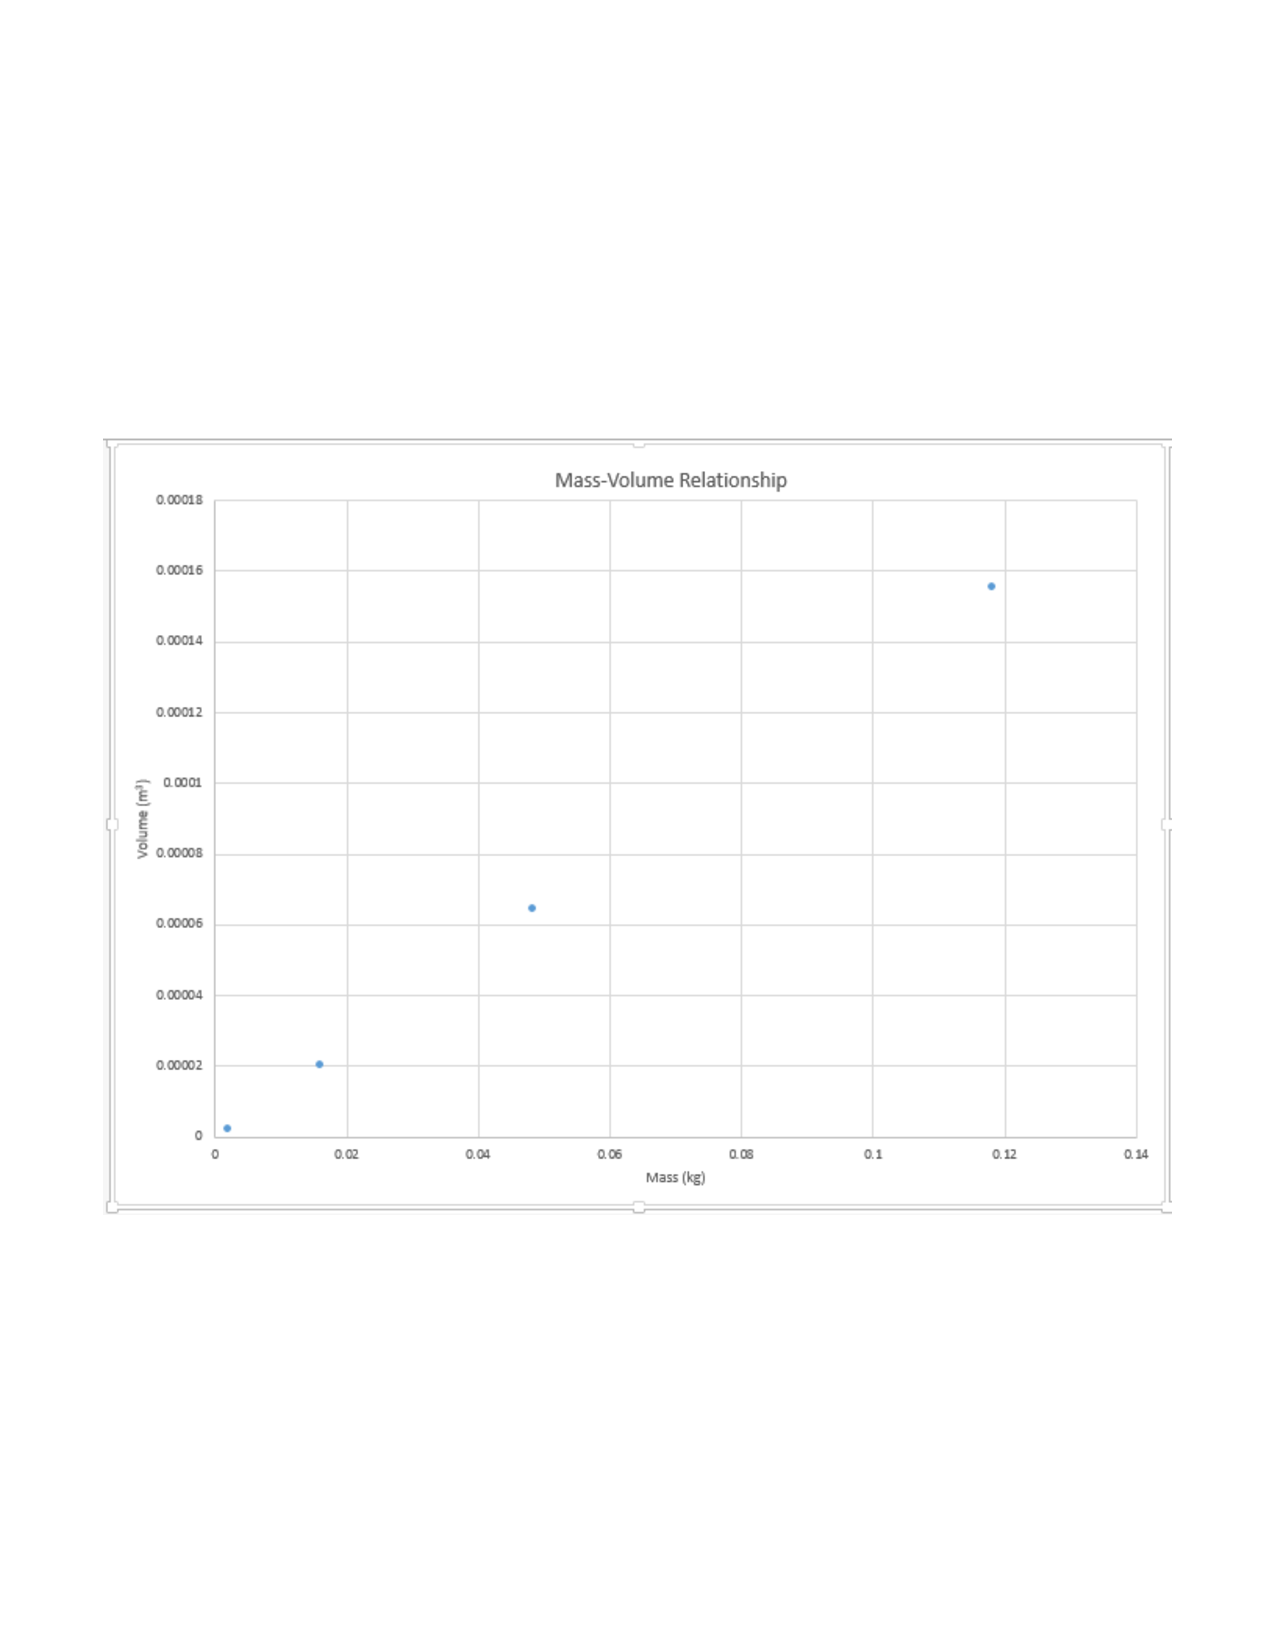
\includegraphics[width=3in]{appendices/excel/excelgraph.pdf}}


Here are a couple of other customizations you may want to do on occasion.
If you double-click on either the horizontal or vertical axis
of your graph, you'll pull up the ``Format Axis'' box. There
are a couple of potentially useful things here. First, you can change
the range of values shown on the graph by
typing numbers into the Minimum and Maximum Bounds boxes.
You can also make the axis run backwards
(with high values on the left / bottom instead of the right / top) by
checking ``Values in reverse order.''
Finally, there's
a checkbox to cause the axis to be 
logarithmic (meaning that the values on it go, say, 1,10,100,1000
instead of 1,2,3,4). 


\subsection{Fitting lines and curves}


After you've made a graph, you can have Excel draw a straight line or
curve that is a best fit to the data.  Select the graph,
then click the $+$ sign at the upper right to bring up the
list of chart elements. Check the ``Trendline'' box.
This should cause a straight line to appear on your graph, which passes
as nearly as possible through the points on the graph.
You can double-click on the line to customize the line
in various ways. One of the most useful is to check the box that says
``Display Equation on chart.''
{\bf Excel will not put the correct units on the numbers in this equation,
but you should.}

\end{document}
